% TU Delft Beamer template
% Author: Maarten Abbink
% Delft University of Technology
% March 2014
% Version 2.0
% Based on original version 1.0 of Carl Schneider
\documentclass{beamer}
\usepackage[english]{babel}
\usepackage{calc}
\usepackage{subfloat}
\usepackage[latin1]{inputenc}
\usefonttheme{professionalfonts}
\usepackage{times}
\usepackage{tikz}
\usepackage{graphicx}
\usepackage{amsmath}
\usepackage{verbatim}
\usetikzlibrary{arrows,shapes}
\usepackage[absolute,overlay]{textpos}
\mode<presentation>{\usetheme{tud}}

\title[Progress Meeting 2]{ Computational Imaging for Earth Surveillance - Progress Meeting  }
%\subtitle
\institute[TU Delft]{Delft University of Technology}
\author{Pranav Sailesh Mani}
\date{March 14, 2017}

% Insert frame before each subsection (requires 2 latex runs)
\AtBeginSubsection[] {
	\begin{frame}<beamer>\frametitle{\titleSubsec}
		\tableofcontents[currentsection,currentsubsection]  % Generation of the Table of Contents
	\end{frame}
}
% Define the title of each inserted pre-subsection frame
\newcommand*\titleSubsec{}
% Define the title of the "Table of Contents" frame
\newcommand*\titleTOC{Outline}

% define a symbol which can be removed if you don't need it
\newcommand{\field}[1]{\mathbb{#1}}
\newcommand{\Zset}{\field{Z}}

\begin{document}
\tikzstyle{every picture}+=[remember picture]
{
% remove the next line if you don't want a background image
\usebackgroundtemplate{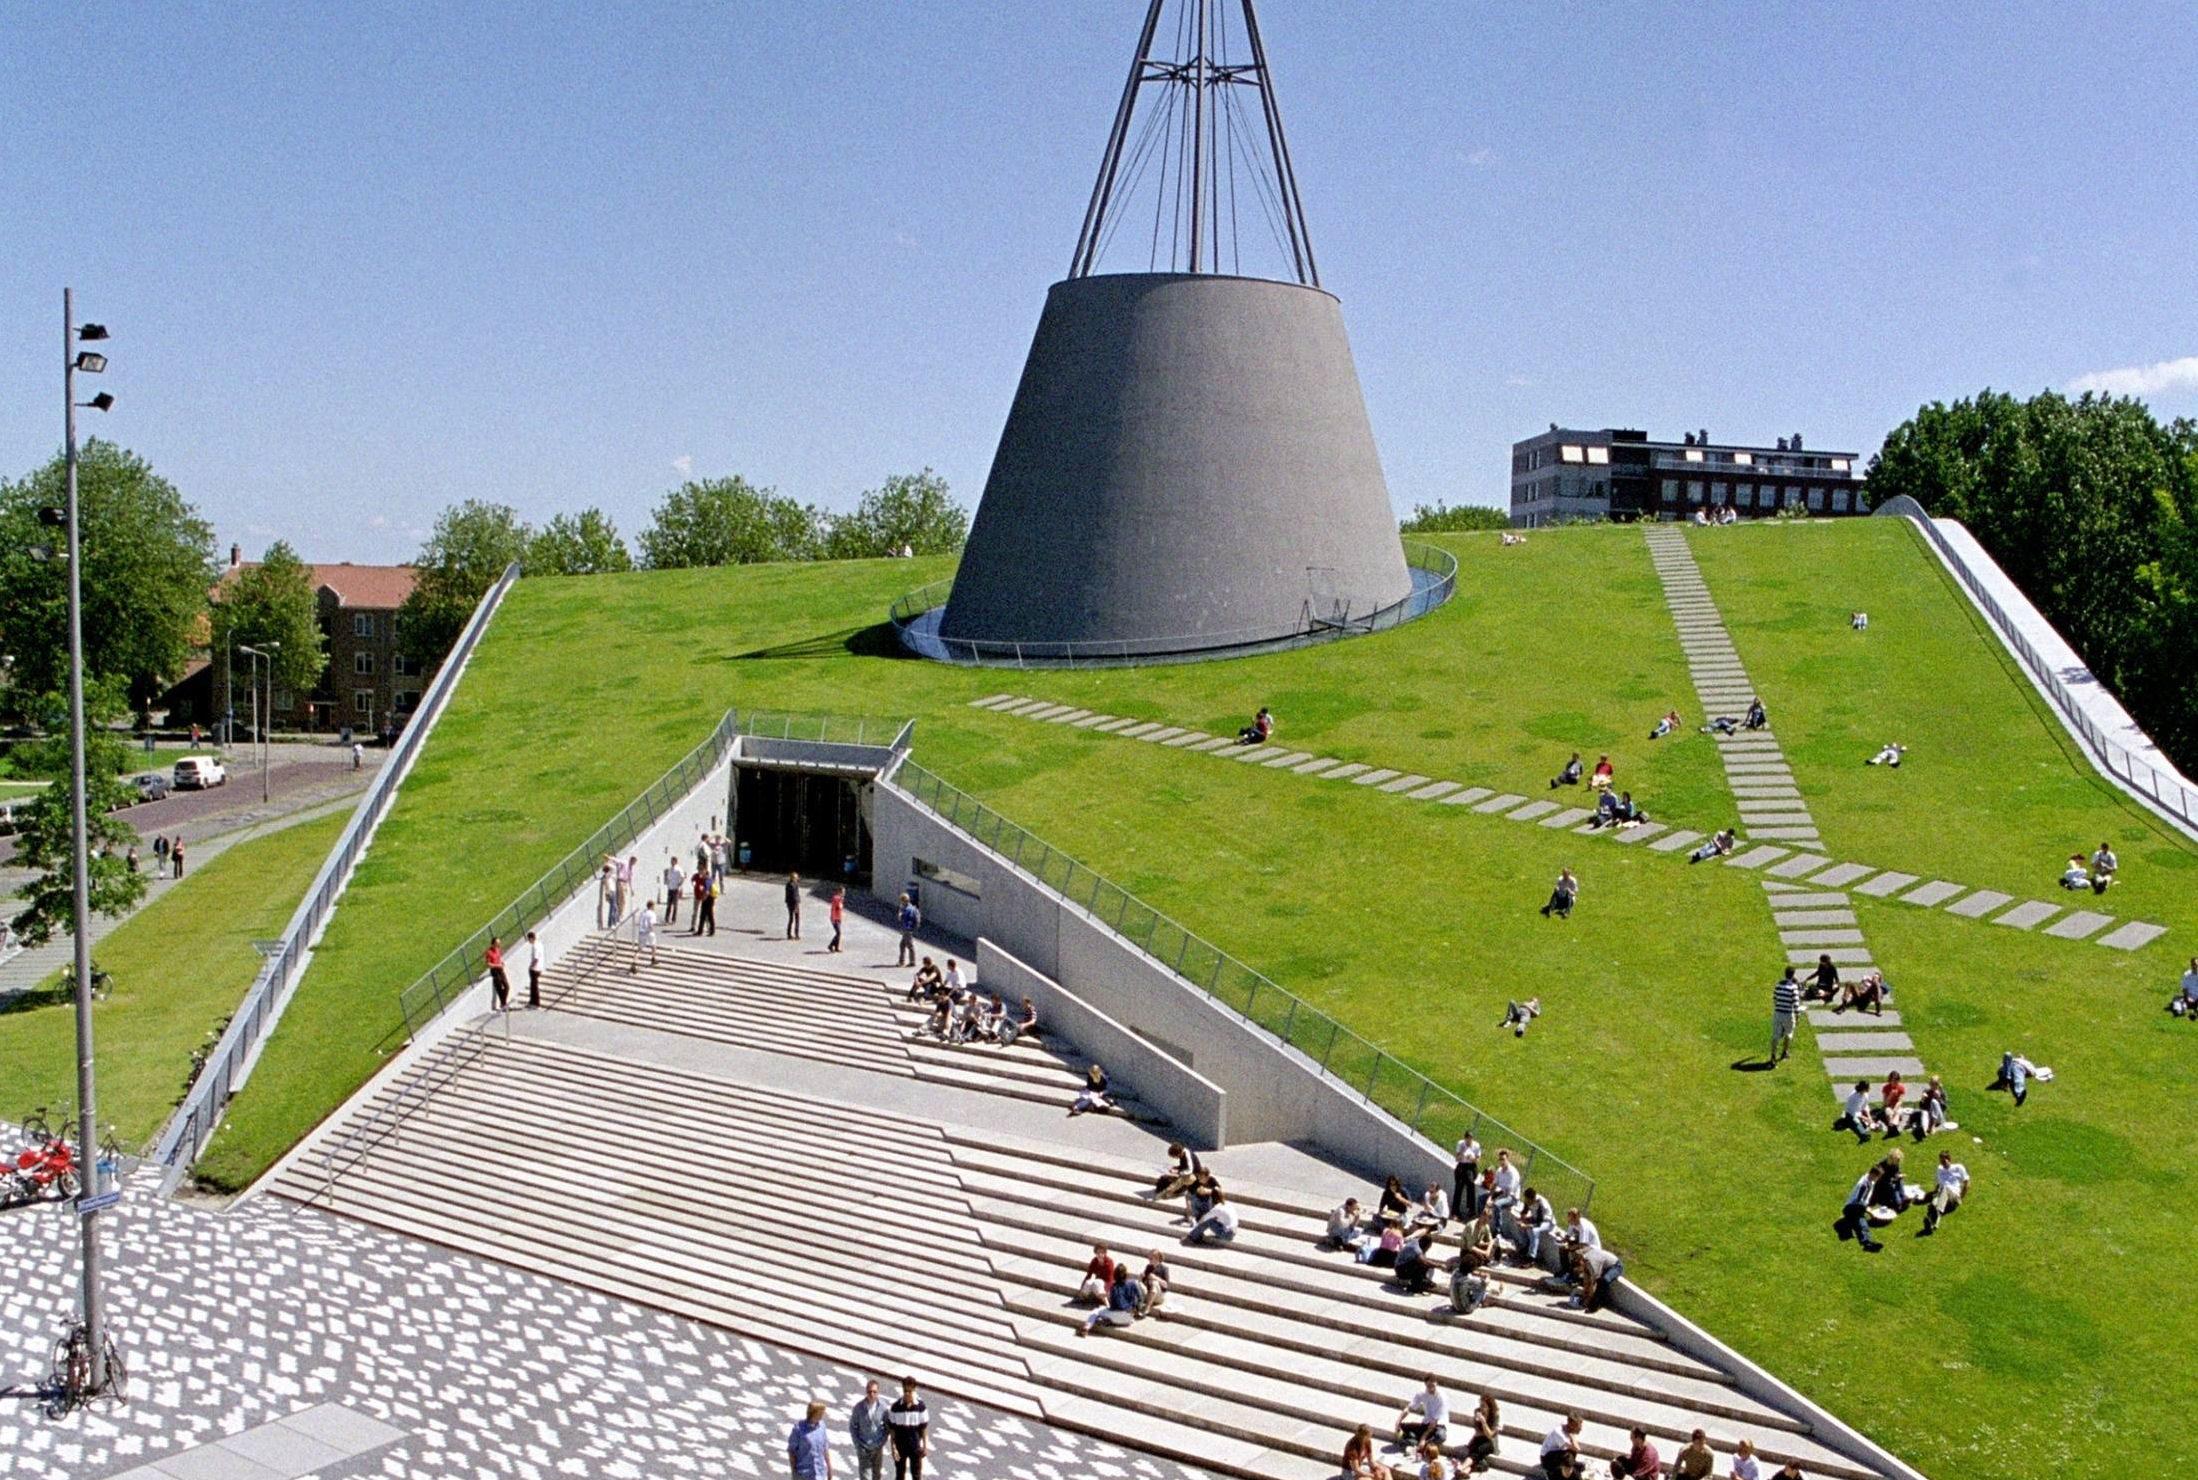
\includegraphics[width=\paperwidth,height=\paperheight]{images/background-titlepage.jpg}}%
\setbeamertemplate{footline}{\usebeamertemplate*{minimal footline}}
\frame{\titlepage}
}

{\setbeamertemplate{footline}{\usebeamertemplate*{minimal footline}}
\begin{frame}\frametitle{\titleTOC}
	\tableofcontents
\end{frame}
}

\section{Objective}
\begin{frame}{Objective}

\begin{itemize}
  \item To design an imaging system for Delfi-PQ satellite satisfying the size and power constraints.
  \item The total system must consume a power of not more than 50mW. The system uses a low power 32-bit microcontroller(MSP432) for processing. 
  \item The size constraints depend on the placement of the camera on the satellite. The total mass of the imager must not exceed 15g.
 
\end{itemize}

\begin{block}{Note}
The aperture can be on the side of the camera or protude through the top. The aperture size cannot exceed 36mm in both ways. The height of the optical part can be 6mm if placed sideways or 12.4mm if placed on the top. 
\end{block}

\end{frame}


\section{Approaches}
\subsection[]{Lensless and Lensed Cameras}
\begin{frame}{Lensless and Lensed Cameras}
\begin{itemize}
\item There are two approaches to this problem- conventional lens based and new class of emerging lensless imaging.
 \item Lensed Cameras are generally bulky, and are suited for the visible light spectrum. The thinnest mobile camera is 5mm thick. The cost of the system goes up if imaging is to be done in  other spectrums.
 \item Lensless cameras can be as small as few hundered microns thick. The trade-off is the computational complexity involved in lensless imaging.
\end{itemize}
\end{frame}
\begin{frame}{Lensless and Lensed Cameras}

\begin{figure}
\centering
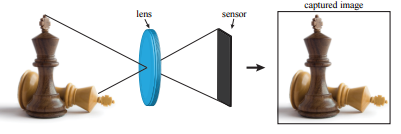
\includegraphics[scale=0.5]{doc_images/lensless_1.PNG}
\caption{Lensed Imaging}
\end{figure}
\begin{figure}
\centering
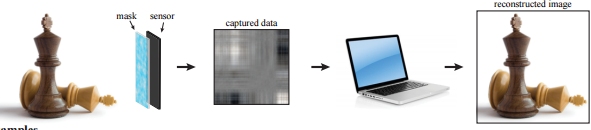
\includegraphics[scale=0.5]{doc_images/lensless_2.PNG}
\caption{Lensless Imaging}
\end{figure}
\end{frame}
\subsection[]{Lensless Cameras}
\begin{frame}{Lensless Cameras}
\begin{itemize}
\item The very first cameras were lensless pinhole cameras.
\item Light passes through a pinhole and forms the image on th e sensor. Very small pinholes are required to produce sharp images. Size of pinhole limits light throughput.
\item Lenses were introduced to increase the size of aperture, increase the sharpness of the image and light throughput.
\item Coded aperture cameras extend the pinhole camera concept replacing the single aperture with a mask containing multiple apertures.
\end{itemize}
\end{frame}
\begin{frame}{Lensless Camera}
\tikzstyle{na} = [baseline=-.5ex]
A lensless camera can be mathematically modelled as\cite{VBoomi}\cite{CannonFenimore1}:
\begin{itemize}
    \item Sensor Measurement
        \tikz[na] \node[coordinate] (n1) {};
\end{itemize}
\begin{equation*}
\tikz[baseline]{
            \node[fill=gray!20,anchor=base](t1){y}} =  \tikz[baseline]{
            \node[fill=blue!20,anchor=base](t2){ {$\phi $}}} * \tikz[baseline]{
            \node[fill=green!20,anchor=base](t3){ {$x $}}} + \tikz[baseline]{
            \node[fill=red!20, ellipse,anchor=base] (t4){e}}
\end{equation*}
\begin{itemize}
\item Mask
 \tikz[na]
 \node [coordinate] (n2) {};
\item Irradiance Vector
 \tikz[na]
 \node [coordinate] (n3) {};
\item Measurement Noise
 \tikz[na]\node [coordinate] (n4) {};
\end{itemize}
\begin{tikzpicture}[overlay]
        \path[->]-> (n1) edge [bend left] (t1);
        \path[->]-> (n2) edge [bend right] (t2);
        \path[->]-> (n3) edge [bend right] (t3);
        \path[->]-> (n4) edge [bend right] (t4);
\end{tikzpicture}
\begin{block}{}
After noise removal, the image can be recovered by using a function that is inverse of the mask. The response of the mask to its inverse is called System Point Spread function. An ideal SPSF would be a $\delta$ function\cite{CannonFenimore1}.
\end{block}
\end{frame}
\subsubsection[]{Fresnel Zone Plates}
\begin{frame}{Fresnel Zone Plates}
\begin{itemize}
\item Introduced by Mertz and Young in the 1960s for a "large aperture, high resolution camera with neither refracting or reflecting components".
\end{itemize}
The FZP is defined such that the radius of the $n^{th}$ zone is given as 
$$
r_n = r_1 \sqrt{n}
$$
and $r_1$ is the radius of the inner most circle.
\end{frame}
\begin{frame}{Fresnel Zone Plates}
\begin{figure}
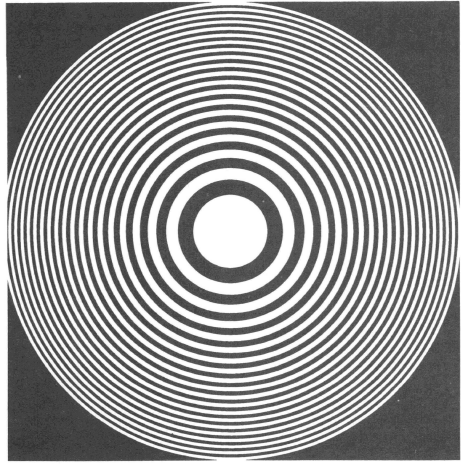
\includegraphics[scale=0.25]{doc_images/lensless_3.PNG}
\caption{Twenty Ring Fresnel Zone Plate}
\end{figure}
\begin{itemize}
\item Zone Plates can be used in place of pinholes or lenses to form an image.
\end{itemize}
\end{frame}
\subsubsection[]{Uniformly Redundant Arrays}
\begin{frame}{Uniformly Redundant Arrays}
\begin{itemize}
\item Developed over the disadvantages associated with random arrays. 
\item Random arrays require infinite apertures to have an ideal SPSF.
\item Fenimore and Cannon developed classes of functions into patterns which are called Uniformly Redundant Arrays with an almost ideal SPF\cite{Fenimore:78}.
\end{itemize}
\begin{figure}{
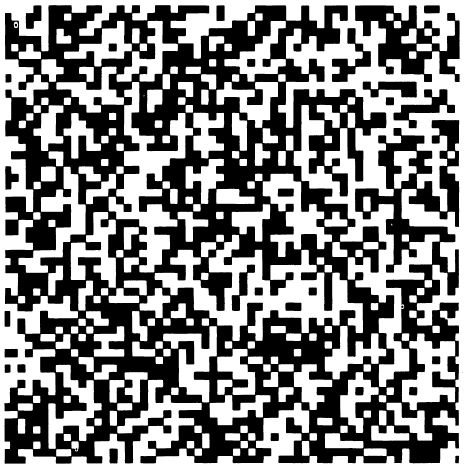
\includegraphics[scale=0.125]{doc_images/lensless_4.PNG}
\caption{A 60 * 60 random array}}
\end{figure}
\end{frame}
\begin{frame}{Uniformly Redundant Arrays}
\begin{figure}{
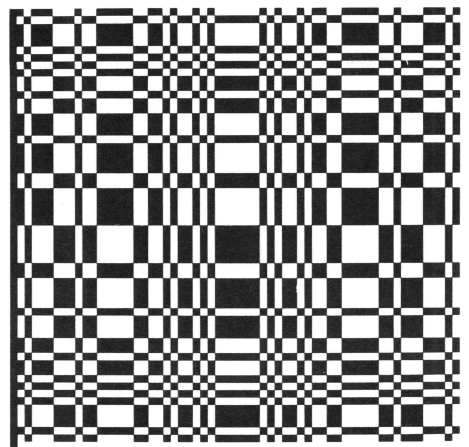
\includegraphics[scale=0.125]{doc_images/lensless_5.PNG}
\caption{A 60 * 59 URA}}
\end{figure}
\begin{itemize}
\item The URA has an ideal response and the open area is approximately 50 percent of that of the total aperture area.
\item The collection efficiency of FZP and the ideal response of the random array is combined.
\end{itemize}
\end{frame}
\subsubsection[]{Doubly Toeplitz Masks}
\begin{frame}{Doubly Toeplitz Masks}
\begin{itemize}
\item The advantage of URA apply only for radiation wavelengths short enough that the diffraction effects are negligible. Reconstruction of images in visible light spectrum results in noisy low-contrast recovered images\cite{Toeplitz}.
\item Doubly Toeplitz masks were designed to solve this problem and reduce the effects of diffraction.
\item The drawback is that the computational complexity increases in the image recovering process.
\end{itemize}
\begin{figure}{

\includegraphics[scale=0.35]{doc_images/lensless_6.PNG}
\caption{Doubly-Toeplitz Mask\cite{Toeplitz}}}
\end{figure}
\end{frame}
\subsubsection[]{FlatCam}
\begin{frame}{FlatCam}
\begin{itemize}
\item The most recent lensless camera architecture\cite{VBoomi}\cite{FlatCam}.
\item Uses pseudo-random maximum length sequence masks which are similar to random arrays. Similar to doubly-toeplitz masks, it places two masks one after the other.
\item Takes an average of 75ms to compute a 512 * 512 image on a standard laptop computer. 10 fps video capture feasible on a PC.
\end{itemize}

\end{frame}
\subsection[]{Lensed Cameras}
\begin{frame}{Lensed Cameras}
\begin{itemize}
\item As mentioned before, they are thicker than lensless camera due to the lenses involved.
\item New designs have come up that considerably reduce the size of the imaging system. 
\end{itemize}
\begin{figure}{
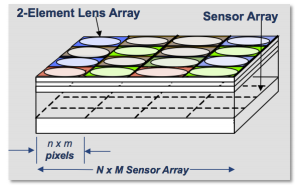
\includegraphics[scale=0.50]{doc_images/lensless_7.PNG}
\caption{PiCam\cite{PiCam}}}
\end{figure}

\end{frame}
\subsubsection[]{PiCam}
\begin{frame}{PiCam}
\begin{itemize}
\item This approach uses multiple small lenses with color filters to capture multiple images
\item Due to multiple CMOS sensors needed for this approach, the power consumption of the camera alone can exceed 500 mW.
\item Apart from this computational reconstruction of the image is required.
\end{itemize}
\begin{figure}
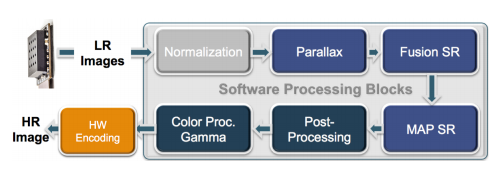
\includegraphics[scale=0.50]{doc_images/lensless_8.PNG}
\caption{PiCam SW Pipeline}
\end{figure}
\end{frame}
\section[]{Conclusion and Next work}
\subsection{Conclusion}
\begin{frame}{Conclusion}
\begin{itemize}
\item Computational Complexity is directly propotional to the power consumed by the MCU for imaging the system.
\item Another approach requires fabricating diffraction grating based CMOS sensors. However, they do not offer any specific advantage compared to the approaches mentioned above.
\item A trade-off needs to be made between the spectrum that needs to be measured and the computational complexity.
\end{itemize}
\begin{table}[ht]
\caption{Comparison of Different Approaches}
\label{tbl:
cmp}
\resizebox{0.75\columnwidth}{!}{
\begin{tabular}{|c|c|c|}
\hline
Approach & Computational Complexity & Spectrum\\
\hline
URA & Low & X-Ray, $\gamma$ Ray \\
\hline
Doubly-Toeplitz & High & Visible, $\gamma$, X-Ray\\
\hline
FlatCam & High & Visible, $\gamma$, X-Ray\\
\hline
PiCam & High & Visible\\
\hline
\end{tabular}}
\end{table}
\end{frame}
\subsection{Next Work}
\begin{frame}{Next Work}
\begin{itemize}
\item Computer based simulation of the approaches mentioned can be done in MATLAB.

\item Acquiring of required CMOS sensors if visible light imaging needs to be done.

\end{itemize}
\end{frame}
\begin{frame}[allowframebreaks]
\frametitle{References}
    {\footnotesize
    \bibliography{bibi}
    \bibliographystyle{ieeetr}
    }
\end{frame}
\end{document}
